\documentclass[main.tex]{subfiles}

\begin{document}

As opposed to the simple DC (direct current) transmission through a conducting wire, AC (alternating current) is usually transmited using transmission cables consisting of coaxial conductors separated by a dielectric. The outer cable is grounded. (figure) Due to electrons changing directions in the wire, current and voltage exhibit wave-like properties, and hence measuring some of these properties is important when considering practical applications. 

In our experiment, we examine how voltage and current behave with respect to varying AC frequencies and varying terminating conditions at the end of the cable (as explained below), and analyze this data to find resonant frequencies, speed of propagation in the cable, and dielectric constant of the insulator - which determines the dielectric material. 

\begin{figure}[H]
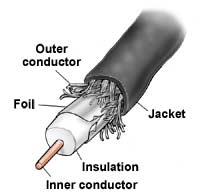
\includegraphics{../data/cable-coaxial.jpg}
\caption{Cross-section of the transmission cable}
\label{cross-cable}
\end{figure}

\end{document}